\begin{figure}[ht]
  	\centering
  	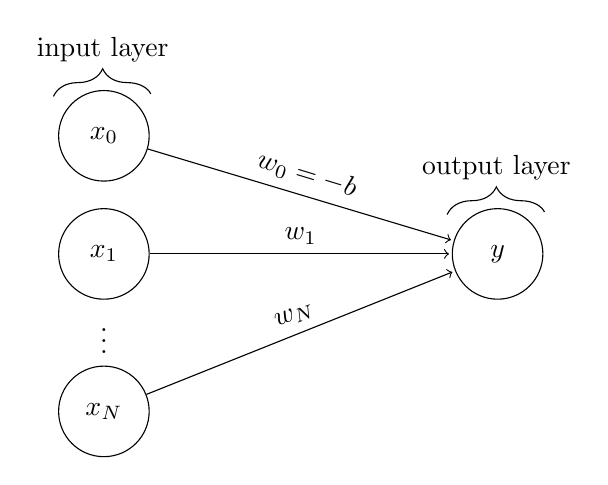
\begin{tikzpicture}[shorten >=1pt]
  	\tikzstyle{unit}=[draw,shape=circle,minimum size=1.15cm]
  	
  	\node[unit](x0) at (0,3.5){$x_0$};
  	\node[unit](x1) at (0,2){$x_1$};
  	\node(dots) at (0,1){\vdots};
  	\node[unit](xn) at (0,0){$x_N$};
  	
  	\node[unit](y1) at (5,2){$y$};
%  	\node(dots) at (4,1.5){\vdots};
%  	\node[unit](yk) at (4,0.5){$y_K$};
  	
  	\draw[->] (x0) -- node[above, rotate = -17]{\( w_0 = -b \)} (y1);
%  	\draw[->] (x0) -- (yk);
  	
  	\draw[->] (x1) -- node[above]{\( w_1 \)}(y1);
%  	\draw[->] (x1) -- (yk);
  	
  	\draw[->] (xn) -- node[above, rotate = 20]{\( w_N \)}(y1);
%  	\draw[->] (xn) -- (yk);
  	
  	\draw [decorate,decoration={brace,amplitude=10pt},xshift=-4pt,yshift=0pt] (-0.5,4) -- (0.75,4) node [black,midway,yshift=+0.6cm]{input layer};
  	\draw [decorate,decoration={brace,amplitude=10pt},xshift=-4pt,yshift=0pt] (4.5,2.5) -- (5.75,2.5) node [black,midway,yshift=+0.6cm]{output layer};
  	\end{tikzpicture}
  	\caption[Network graph of a perceptron with $N$ input units.]{The perceptron consists of $N$ input units and at least one output unit. All units are labeled according to their output: $y = H(z)$ in the case of the output unit; $x_n$ in the case of input units. The input values $x_n$ are propagated to the output unit using a weighted sum, in other words \( z = \bm w^{\intercal}\bm x \). An additional input value $x_0 := 1$ is used to include the biases as weights.}
  	\label{fig:perceptron}
\end{figure}